To evaluate the models introduced in the previous section we conducted a study with human participants.
The study aimed to answer two research questions: ``Can a virtual agent use our  models to shape the footing of participants in multiparty interactions in virtual reality?'' and ``Does the display type (e.g. VR or on-screen) influence the effects?''

In our study, human participants engaged in short, 10-minute conversations with a virtual agent and a simulated, avatar-embodied confederate. The virtual agent displayed gaze behaviors and body orientation that would either include the participant as an addressee or exclude them as a bystander. The goal of this manipulation was to show that participants would conform to the conversational role signaled by the agent using our behavior models---e.g., when assigned the role of bystanders, participants would converse less with the agent.

While our models are independent of the display type used, we expect that the effects of the models will be stronger when the interaction is experiences in VR. A VR application using a head-mounted display provides improved affordances over a desktop display, such as a wide field of view and natural control of viewpoint, which may strengthen the perception of social cues. Therefore, we expect people to be more sensitive to behaviors displayed by agents within an immersive VR environment.
To test this, our experiment manipulates display type to compare a VR headset (Oculus Rift CV1) with a desktop display.

\subsection{Hypotheses}

Our evaluation tested the following hypotheses.

\subsubsection{Hypothesis 1}

Participants will demonstrate conversational behavior that conforms to the footing signaled by the agent's gaze and spatial orientation cues. Specifically, participants in addressee roles will speak more. This is consistent with research on human conversational behavior, which shows that conversing partners tend to orient themselves in an F-formation~\cite{kendon1990conducting} and that people tend to look toward the addressees of their utterances~\cite{kendon1967some}.

\subsubsection{Hypothesis 2}

Participants in addressee roles will feel more groupness and closeness with the agent, as well as evaluate the agent more positively than those in bystander roles. This is based on findings that people report negative feelings about a group and its members when being ignored or excluded~\cite{geller1974being}.

\subsubsection{Hypothesis 3}

The agent's footing cues will have a stronger effect on the participants' conversational behavior (Hypothesis 1) in the VR setting than when using a 2D display.

\subsubsection{Hypothesis 4}

The agent's footing cues will have a stronger effect on the participants' subjective perceptions of the agent and their feelings of closeness and groupness (Hypothesis 2) in the VR setting than when using a 2D display.

Hypotheses 3-4 are based on the premise that the increased affordances of VR will lead to a stronger sense of the agent's social presence and heightened awareness of their nonverbal signals, relative to presentation on a traditional display. Virtual reality provides stereo depth cues, a wide field of view, and natural control over viewpoint. All of these may augment participants' perceptions of the agent and its behaviors.

\subsection{Study Design}

The study followed a mixed, $2 \times 2$ factorial design. The independent variables were \emph{agent behavior} (between-participants) and \emph{task setting} (within-participants). The agent behavior variable had the following levels:

\begin{enumerate}
\item \emph{Exclusive} -- The agent displayed nonverbal behaviors that excluded the participant from the interaction, treating them as a bystander. It oriented its body toward the confederate (facing them straight-on) and gazed at them much more than at the participant, in accordance with the distributions given in Table~\ref{tab:GazeFootingSpatial}.
\item \emph{Inclusive} -- The agent displayed nonverbal behaviors that included the participant in the interaction as an addressee. It distributed its body orientation evenly between the participant and the confederate (using the mechanism depicted in Figure~\ref{fig:FTorsoAlign}) and gazed toward them equally (Table~\ref{tab:GazeFootingSpatial}).
\end{enumerate}

\begin{figure}
\centering
\includegraphics[width=1\textwidth]{conversationalrolegaze/Figures/GazeFootingConditions.pdf}
\caption{Conditions of the \emph{agent behavior} independent variable. Upper row: conversational formation. Bottom row: participant's view of the scene.}
\label{fig:GazeFootingConditions}
\end{figure}

Figure~\ref{fig:GazeFootingConditions} illustrates the agent behavior manipulation. The upper row of images show the conversational formations resulting from agent's body orientation shifts at each level of the manipulation, whereas the bottom images show the views of the scene from the participant's perspective.

The other independent variable, task setting, had the following levels:

\begin{enumerate}
\item \emph{2D display} -- The participant experienced the interaction on a 27'' Dell monitor, at $2560 \times 1440$ resolution and a field of view of 50$^\circ$, while using the mouse to control the viewpoint.
\item \emph{VR} -- The participant wore a VR headset (Oculus Rift CV1). They saw the scene at the resolution of $1080 \times 1200$ per eye, with a 110$^\circ$ field of view. Built-in head orientation tracking and the external positional tracker allowed the participant to control the viewpoint by moving their head.
\end{enumerate}

The two task setting conditions were designed to approximate the standard or expected usage of interactive, virtual agent systems. The \emph{2D display} condition approximated the experience of a 3D, first-person game or virtual world on a personal computer with a single display, which represents the state of the art for the majority of users. The FOV value of 50$^\circ$ is fairly standard in 3D applications; distance magnification and perspective distortion effects become noticeable at values above 60$^\circ$. The use of the Oculus Rift in the \emph{VR} condition afforded a much higher field of view and more natural viewpoint control, allowing the participant to easily see both the agent and the confederate simultaneously, as well as shift their gaze from one to the other by simply moving their head. The screenshots in Figure~\ref{fig:GazeFootingConditions} are both from the \emph{2D display} condition.

Since the study had a within-participants factor (\emph{task setting}), we implemented two versions of the task to reduce transfer effects. The participants were assigned to conditions in a stratified order, counterbalanced with respect to task setting (\emph{2D display} or \emph{VR}) and task version (\emph{Task 1} or \emph{Task 2}).

\subsection{Task}

\begin{figure}
\centering
\includegraphics[width=1\textwidth]{conversationalrolegaze/Figures/GazeFootingTask.pdf}
\caption{Left: the participant's view of the scene at the start of the task. Right: physical task setup.}
\label{fig:GazeFootingTask}
\end{figure}

The study task was a three-party interaction in a virtual room. The interaction took the form of a casual, interview-style conversation moderated by the agent. Both task versions had the same structure and length, but they differed in content---the agent asked a different set of questions in each task. Her name and appearance were also changed to suggest that this was a different agent.

The conversational partners were the agent, the participant, and a ``simulated confederate''---a human-voiced agent which produced prerecorded utterances, but the participants were led to believe it was a real human in another room. At the start of the task, the participant found themselves standing at the room's entrance with a view of the agent and confederate on the other side of the room (Figure~\ref{fig:GazeFootingTask}, left); the agent and confederate faced each other in a vis-a-vis formation. The participant was prompted to click a button (either on the mouse or the Oculus Remote) to initiate the interaction; upon doing so, the camera automatically approached the group. Depending on the agent behavior condition, the agent either briefly glanced toward the participant and continued facing the confederate (\emph{exclusive} agent behavior) or reoriented herself toward the participant (\emph{inclusive} agent behavior).

After introducing herself and greeting the partners, the agent began asking casual questions about the partners' life experiences and interests. Some questions were designed to elicit short, one-sentence responses (e.g., ``What is your favorite movie?''), while others elicited longer, more open-ended responses (e.g., ``What is your favorite movie about?'') Most questions were implicitly addressed at both the participant and confederate, who both had a choice in answering them. We expected that the participant was more likely to take the conversational floor and answer the question if the agent demonstrated inclusive nonverbal behaviors.

At the end of the agent's turn, the system randomly decided if the confederate should answer the current question or not. If yes, the confederate took the floor within about 0.75 $s$ and gave a prerecorded response to the question. If not, the system waited 3.4 $s$ for someone to speak out; if no one did, either the confederate took the floor and answered, or the agent proceeded with the next question. The pause values between turns were derived from measurements of human speech in prior work and padded for possible speech recognition lag. According to Weilhammer~\citep{weilhammer2003durational}, the mean pause between turns is about 380 $ms$ in spontaneous American-English discourse, whereas silences longer than 3 $s$ are experienced as uncomfortable~\citep{mclaughlin1982awkward}.

\subsubsection{Setup}

The physical setup of the task is shown in Figure~\ref{fig:GazeFootingTask}, right. Participants were seated in an office chair in front of a personal computer while wearing an audio headset (in the \emph{2D display} condition) or Oculus Rift (in the \emph{VR} condition). A video camera was set up to record their behavior.

\subsubsection{Implementation}

The task was implemented in Unity game engine and utilized the embodied dialog system described in the previous section. The task logic and measurements were implemented in C\# scripts. The confederate's lip movements were animated using Oculus Lip Sync. The agent and confederate character models were imported from DAZ\footnote{DAZ Productions, http://www.daz3d.com/}. Their visual design was deliberately stylized in order to reduce uncanny valley effects~\citep{mori2012uncanny}, though their proportions were sufficiently realistic that gaze motion adaptation (using methods from Chapter~\ref{cha:StylizedGaze}) was unnecessary. Both models had a looping, idle body animation applied to enhance the naturalness of their behavior.

\subsection{Participants}

We recruited 32 participants (17 female and 15 male) through an online student job website as well as in-person from a university campus. All participants were students. Twenty-seven participants were native English speakers.

\subsection{Procedure}

We conducted the experiment in a study room with no outside distraction. The participants were ushered into the room by the experimenter and seated at the table. Following a brief overview of the task, they were given a consent form to read and sign. Next, they were given verbal task instructions and handed a printed instructions sheet to serve as a reminder. The experimenter then launched the task application and left the room. Upon task completion, the participants filled out a questionnaire for subjective evaluation of the agent and task. Next, the participants performed a second trial of the task, upon which they filled out another subjective questionnaire and a brief demographics questionnaire. Finally, the participants received payment in the amount of \$5. Total experiment duration was 30 minutes.

\subsection{Measures}

The experiment involved two behavioral and several subjective measures. The behavioral measures were designed to measure the participants' level of participation in the interaction, in order to test hypotheses 1 and 3. They were the following:

\begin{enumerate}
\item \emph{Number of speaking turns} -- Total number of speaking turns taken by the participant over the course of the interaction.
\item \emph{Total speaking time} -- Cumulative length (in seconds) of the participant's speaking utterances over the course of the interaction.
\end{enumerate}

When calculating the behavioral measures, we excluded participants' responses to the first five questions (out of twenty-five total) to account for high variability due to acclimation.

The subjective measures were collected using the subjective questionnaire and consisted of seven-point scale items. The measures were the following:

\begin{enumerate}
\item To measure the agent's likeability, we asked participants to rate the agent on nine traits such as likeability, cuteness, and friendliness. From this data, we constructed a scale consisting of two factors: \emph{likeability} (two items, Cronbach's $\alpha = 0.824$) and \emph{attractiveness} (three items, Cronbach's $\alpha = 0.929$).
\item Feelings of \emph{closeness} to the agent were measured using a four-item scale (Cronbach's $\alpha = 0.823$) adapted from~\citet{aron1992inclusion}, who asked participants to indicate their agreement with statements such as ``The agent paid attention to me.''
\item Groupness was measured using a scale adapted from~\citet{williams2000cyberostracism}, which consisted of seven items (Cronbach's $\alpha = 0.827$) and asked participants to indicate their agreement with statements such as ``I felt ignored or excluded by the group.''
\end{enumerate}

The questionnaire also included a check for the agent behavior manipulation, implemented as a two-item scale: (1) ``The agent faced me during the interaction'' and (2) ``The agent faced the other participant.''

\subsection{Results}

Having collected our data, we first performed a one-way analysis of variance (ANOVA) on the manipulation check scale. We found a significant effect of agent behavior on the manipulation check, $F(1, 61) = 5.743, p = .0196$.

\subsubsection{Behavioral Measures}

\begin{figure}
\centering
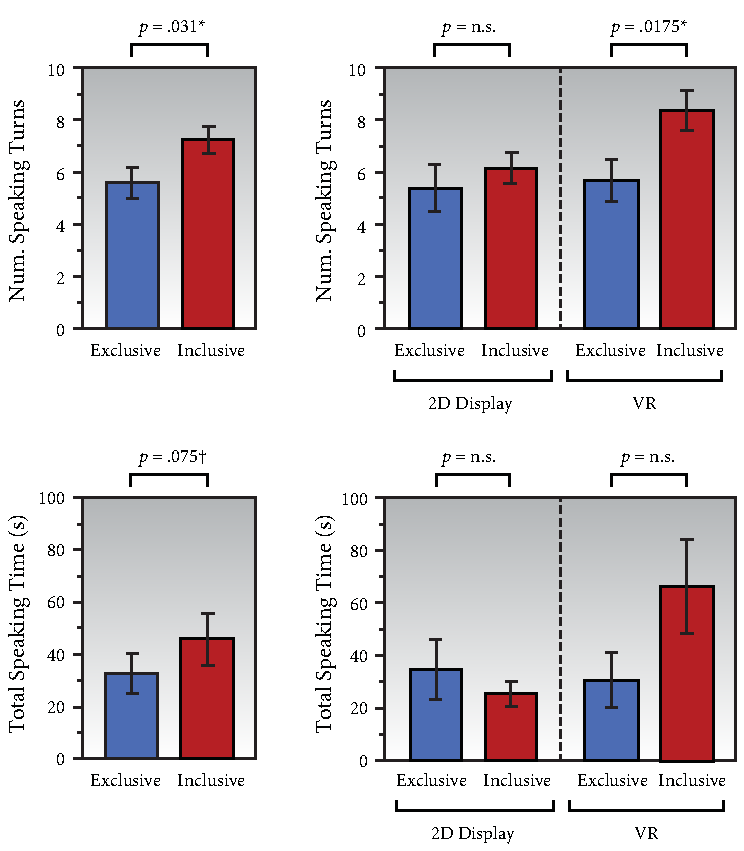
\includegraphics[width=0.95\textwidth]{conversationalrolegaze/Figures/ResultsBehavioral.pdf}
\caption{Results from behavioral measures. Left: number of speaking turns (top) and total speaking time (bottom) by agent behavior (\emph{exclusive} vs. \emph{inclusive}). Right: same measures by agent behavior and task setting (\emph{2D display} vs. \emph{VR}). ($*$) denotes a significant effect, while ($\dagger$) denotes a marginal effect.}
\label{fig:GazeFootingResultsBehavioral}
\end{figure}

Next, we analyzed our behavioral measures with a two-way, mixed-design ANOVA. We found a marginal main effect of agent behavior on the \emph{number of speaking turns} ($F(1, 30) = 3.757, p = .062$) and no effect of agent behavior on the \emph{total speaking time} ($F(1, 30) = 1.159, p = .290$). These findings provide partial support for Hypothesis 1.

We found no interaction between agent behavior and task setting on the \emph{number of speaking turns} ($F(1, 30) = 2.217, p = .147$). However, we did find a marginal interaction between agent behavior and task setting on the \emph{total speaking time} ($F(1, 30) = 3.637, p = .066$). Furthermore, we found a simple effect of agent behavior on the number of speaking turns in the \emph{VR} setting; the number of turns taken in the \emph{inclusive} condition was significantly higher than in the \emph{exclusive} condition (5.7 versus 8.4), $F(1, 55) = 5.970, p = .0178)$. No such effect of the agent behavior manipulation was found in the \emph{2D display} setting, $F(1, 55) = 0.465, p = .498$. An equivalent set of comparisons for the speaking time measure found a marginal effect of agent behavior manipulation in the \emph{VR} setting ($F(1, 59) = 3.472, p = .0387$). No such effect of agent behavior was found in the \emph{2D display} setting ($F(1, 59) = 0.287, p = .594$). All the pairwise comparisons were performed at a Bonferroni-corrected alpha level of $.025$. These findings provide support for Hypothesis 3.

Additionally, we confirmed that \emph{task version} had no significant effect on either the number of speaking turns ($F(1, 62) = 0.001, p = .970$) or total speaking time ($F(1, 61) = 0.235, p = .630$), suggesting the two tasks were sufficiently similar for our purposes.

\subsubsection{Subjective Measures}

To analyze the subjective measures, we performed a two-way, mixed-design ANOVA. We found no main effects of agent behavior on any of our subjective measures: \emph{likeability} ($F(1, 30) = 0.363, p = .551$), \emph{attractiveness} ($F(1, 30) = 1.719, p = .200$), \emph{closeness} ($F(1, 30) = 0.606, p = .443$), or \emph{groupness} ($F(1, 30) = 0.140, p = .711$). We also found no significant interactions of agent behavior and task setting on any of the subjective measures: \emph{likeability} ($F(1, 30) = 1.233, p = .276$), \emph{attractiveness} ($F(1, 30) = 0.417, p = .243$), \emph{closeness} ($F(1, 30) = 0.092, p = .764$), \emph{groupness} $(F(1, 30) = 0.086, p = .771$). We conclude that hypotheses 2 and 4 are not supported by these results.

\begin{figure}
\centering
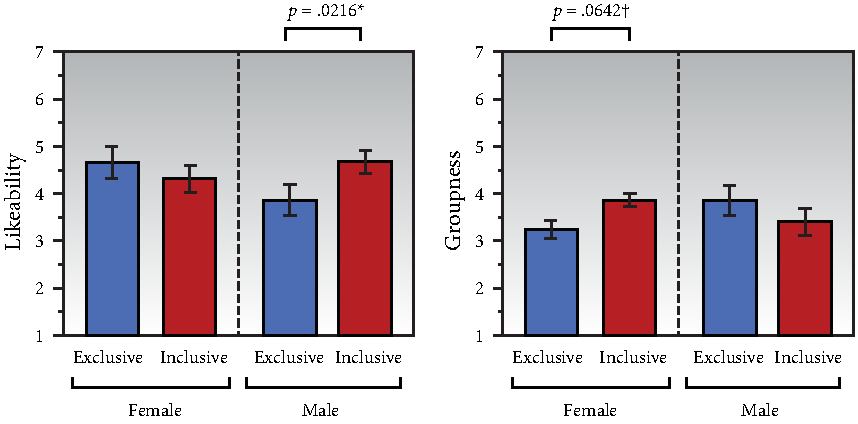
\includegraphics[width=1\textwidth]{conversationalrolegaze/Figures/ResultsSubjectiveGender.pdf}
\caption{Results from two subjective measures (likeability and groupness) by agent behavior (\emph{exclusive} vs. \emph{inclusive}) and participant gender. ($*$) denotes a significant effect, while ($\dagger$) denotes a marginal effect.}
\label{fig:GazeFootingSubjectiveGender}
\end{figure}

In a post-hoc analysis, we analyzed the effects of participant gender on our measures, since prior work~\citep{mutlu2006storytelling,bailenson2001equilibrium} suggests that men and women may respond differently to the gaze behavior of humanlike agents. We found a significant, cross-over interaction between agent behavior and participant gender on the \emph{likeability} measure, $F(1, 60) = 5.885, p = .0183$ (Figure~\ref{fig:GazeFootingSubjectiveGender}, left). A pairwise comparison showed that male participants rated the agent exhibiting inclusive behavior significantly higher than when exhibiting exclusive behavior ($F(1, 60) = 5.561, p = .0216$), which suggests that the effects predicted by Hypothesis 2 may be observed in male participants. We also found a significant interaction of agent behavior and gender on the \emph{groupness} measure, $F(1, 60) = 4.988, p = .0293$ (Figure~\ref{fig:GazeFootingSubjectiveGender}, right). Female participants assigned marginally higher groupness ratings to the agent exhibiting inclusive behavior than the one displaying exclusive behavior, $F(1, 60) = 3.554, p = .0642$.

\subsection{Discussion}

The study results suggest that the footing behavior models introduced in our work enable a virtual agent to use its gaze and body orientation to shape the conversational roles of human users, but only in an immersive VR setting. However, there is less evidence that the use of these cues improves users' subjective experiences of the interaction, other than higher likeability ratings of the agent given by male participants and a marginal improvement in the feelings of groupness of the female participants.

Some of the effects of our manipulations were not as strong as expected, possibly due to limitations of the dialog system and the agent's behaviors. A common issue with speech-based dialog systems is the lagging of speech recognition results behind the participant's speech production. This issue, compounded with some participants' tendency to pause between utterances, sometimes caused our system to interpret a gap between incoming speech recognition results as floor release and cut off the participant. Interrupting the participant would have had a direct effect on the speaking time measure and might have reduced it substantially.
Furthermore, the effects of the agent's footing signals might have been partially confounded by other aspects of the agent's and confederate's behavior. For example, both the agent and confederate embodiments only had a looping body animation and displayed no body movements connected to the discourse, such as hand gestures. While the simplicity of their overall behavior is advantageous from the standpoint of experimental control, it could have also seemed unnatural and distracting to participants.

Finally, the interaction effects between the agent's behavior and participant gender are not unexpected. For example,~\citet{mutlu2006storytelling} reported that female participants responded more negatively to increased gaze from a humanlike robot. They speculated that this phenomenon was linked to findings by~\citet{bailenson2001equilibrium}, which suggest that women tend to maintain greater interpersonal distance than men from a virtual agent displaying increased mutual gaze. Since interpersonal distance between participants and the agent was constant in our experiment, high mutual gaze from the agent might have had negative effects in female participants. Further experimentation is required to test this hypothesis. 